\documentclass{article}

\usepackage{amsmath}
\usepackage{amssymb}
\usepackage{graphicx}

\begin{document}
\title{\LARGE Assignment 4}
\author{Jianqiang DU\\\\017547307}
\maketitle

\section{Exercise 7.4: (c), (g), (h), and (j) with justifications}
\begin{itemize}
\item[Q:]Which of the following are correct?
\begin{itemize}
\item[(c)]$(\textit A \wedge \textit B) \models (\textit A \Leftrightarrow \textit B)$.
\item[(g)]$(\textit C \vee (\neg \textit A \wedge \neg \textit B)) \equiv ((\textit A \Rightarrow \textit C) \wedge (\textit B \Rightarrow \textit C))$.
\item[(h)]$(\textit A \vee \textit B) \wedge (\neg \textit C \vee \neg \textit D \vee \textit E) \models (\textit A \vee \textit B)$.
\item[(j)]$(\textit A \vee \textit B) \wedge \neg (\textit A \Rightarrow \textit B)$ is satisfiable.
\end{itemize}
\item[A:]
\begin{itemize}
\item[(c)]Correct. If $(\textit A \wedge \textit B)$ is true, then \textit A must be true and \textit B must be true, then $(\text A \Leftrightarrow \textit B)$ must be true, thus $(\textit A \wedge \textit B) \models (\textit A \Leftrightarrow \textit B)$ is correct.
\item[(g)]Correct.\\$((\textit A \Rightarrow \textit C) \wedge (\textit B \Rightarrow \textit C))$\\$\equiv (\neg \textit A \vee \textit C) \wedge (\neg \textit B \vee \textit C)$\\$\equiv (\textit C \vee \neg \textit A) \wedge (\textit C \vee \neg \textit B)$\\$\equiv (\textit C \vee (\neg \textit A \wedge \neg \textit B))$
\item[(h)]Correct. If $(\textit A \vee \textit B) \wedge (\neg \textit C \vee \neg \textit D \vee \textit E)$ is true, then $(\textit A \vee \textit B)$ is true and $(\neg \textit C \vee \neg \textit D \vee \textit E)$ is true, then $(\textit A \vee \textit B) \wedge (\neg \textit C \vee \neg \textit D \vee \textit E) \models (\textit A \vee \textit B)$ is correct.
\item[(j)]Satisfiable when \textit A is true and \textit B is false.\\$(\textit A \vee \textit B) \wedge \neg (\textit A \Rightarrow \textit B)$\\$\equiv (\textit A \vee \textit B) \wedge \neg (\neg \textit A \vee \textit B)$\\$\equiv (\textit A \vee \textit B) \wedge (\textit A \wedge \neg \textit B)$\\$\equiv (\textit A \vee \textit B) \wedge \textit A \wedge \neg \textit B$
\end{itemize}
\end{itemize}

\section{Exercise 7.6: (b) with justification}
\begin{itemize}
\item[Q:]Prove, or find a counterexample to, each of the following assertions:
\begin{itemize}
\item[(b)]If $\alpha \models (\beta \wedge \gamma)$ then $\alpha \models \beta$ and $\alpha \models \gamma$.
\end{itemize}
\item[A:]Prove
\begin{itemize}
\item[(b)]If $\alpha$ is true, then $(\beta \wedge \gamma)$ is true, then $\beta$ must be true and $\gamma$ must be true, thus $\alpha \models \beta$ and $\alpha \models \gamma$.
\end{itemize}
\end{itemize}


\section{Prove $[(\textit F \Rightarrow \textit P) \vee (\textit D \Rightarrow \textit P)] \equiv [(\textit F \wedge \textit D) \Rightarrow \textit P]$ by converting them into CNF separately}
\begin{itemize}
\item[ ]$[(\textit F \Rightarrow \textit P) \vee (\textit D \Rightarrow \textit P)]$\\$\equiv (\neg \textit F \vee \textit P) \vee (\neg \textit D \vee \textit P)$\\$\equiv \neg \textit F \vee \neg \textit D \vee \textit P$\\$\equiv \neg (\textit F \wedge \textit D) \vee \textit P$\\$\equiv (\textit F \wedge \textit D) \Rightarrow \textit P$
\end{itemize}

\section{Exercise 13.3: (a)}
\begin{itemize}
\item[Q:]For each of the following statements, either prove it is true or give a counterexample.
\begin{itemize}
\item[(a)]If \textit P(\textit a $\vert$ \textit b, \textit c) = \textit P(\textit b $\vert$ \textit a, \textit c), then \textit P(\textit a $\vert$ \textit c) = \textit P(\textit b $\vert$ \textit c)
\end{itemize}
\item[A:]Prove
\begin{itemize}
\item[(a)]$\because \textit P(\textit a \vert \textit b, \textit c) = \textit P(\textit b \vert \textit a, \textit c)$\\$\therefore \frac{\textit P(\textit a \wedge \textit b \wedge \textit c)}{\textit P(\textit b \wedge \textit c)} = \frac{\textit P(\textit b \wedge \textit a \wedge \textit c)}{\textit P(\textit a \wedge \textit c)}$\\$\therefore \textit P(\textit b \wedge \textit c) = \textit P(\textit a \wedge \textit c)$\\$\therefore \frac{\textit P(\textit b \wedge \textit c)}{\textit P(\textit c)} = \frac{\textit P(\textit a \wedge \textit c)}{\textit P(\textit c)}$\\$\therefore \textit P(\textit b \vert \textit c) = \textit P(\textit a \vert \textit c)$
\end{itemize}
\end{itemize}

\section{Exercise 13.8: (a), (b), (c)}
\begin{itemize}
\item[Q:]Given the full joint distribution shown in Figure 13.3, calculate the following:
\begin{figure}[h!]
\centering
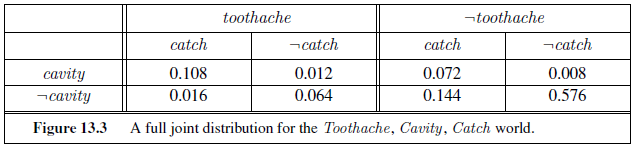
\includegraphics[width=\textwidth]{fig13_3.png}
\end{figure}
\begin{itemize}
\item[(a)]\textbf P(\textit{toothache}).
\item[(b)]\textbf P(\textit{Cavity}).
\item[(c)]\textbf P(\textit{Toothache $\vert$ cavity}).
\end{itemize}
\item[A:]
\begin{itemize}
\item[(a)]\textbf P(\textit{toothache}) = 0.108 + 0.012 + 0.016 + 0.064 = 0.2
\item[(b)]\textbf P(\textit{Cavity}) = \textbf P(\textit{cavity $\vee$ $\neg$cavity}) = 0.108 + 0.012 + 0.072 + 0.008 + 0.016 + 0.064 + 0.144 + 0.576 = 1
\item[(c)]\textbf P(\textit{Toothache $\vert$ cavity}) = $\alpha\langle\textbf P(\textit{toothache}\wedge\textit{cavity}),\textbf P(\neg\textit{toothache}\wedge\textit{cavity}\rangle$\\= $\alpha\langle0.108 + 0.012, 0.072 + 0.008\rangle$\\ = $\alpha\langle0.12, 0.08\rangle$\\$\because\alpha$(0.12 + 0.08) = 1\\$\therefore\alpha$ = 5\\\textbf P = 5$\langle$0.12, 0.08$\rangle$ = $\langle$0.6, 0.4$\rangle$
\end{itemize}
\end{itemize}

\section{Exercise 13.16:}
\begin{itemize}
\item[Q:]It is quite often useful to consider the effect of some specific propositions in the context of some general background evidence that remains fixed, rather than in the complete absence of information. The following questions ask you to prove more general versions of the product rule and Bayes' rule, with respect to some background evidence e:
\begin{itemize}
\item[a.]Prove the conditionalized version of the general product rule:\\\textbf P(\textit X, \textit Y $\vert$ e) = \textbf P(\textit X $\vert$ \textit Y, e)\textbf P(\textit Y $\vert$ e).
\item[b.]Prove the conditionalized version of Bayes' rule in Equation (13.13).
\end{itemize}
\item[A:]
\begin{itemize}
\item[a.]\textbf P(\textit X, \textit Y $\vert$ e) = $\frac{\textbf P(\textit X, \textit Y, e)}{\textbf P(e)}$ = $\frac{\textbf P(\textit X \vert \textit Y, e) \textbf P(\textit Y, e)}{\textbf P(e)}$ = \textbf P(\textit X $\vert$ \textit Y, e)\textbf P(\textit Y $\vert$ e)
\item[b.]\textbf P(\textit Y $\vert$ \textit X, e) = $\frac{\textbf P(\textit Y, \textit X, e)}{\textbf P(\textit X, e)}$ = $\frac{\textbf P(\textit X, \textit Y, e)}{\textbf P(\textit X, e)}$\\=$\frac{\textbf P(\textit X \vert \textit Y, e)\textbf P(\textit Y \vert e)}{\textbf P(\textit X, e)}$ = $\frac{\textbf P(\textit X \vert \textit Y, e)}{\frac{\textbf P(\textit X \vert e)}{\textbf P(e)}}$$\frac{\textbf P(\textit Y \vert e)}{\textbf P(e)}$ = $\frac{\textbf P(\textit X \vert \textit Y, e)\textbf P(\textit Y \vert e)}{\textbf P(\textit X \vert e)}$
\end{itemize}
\end{itemize}

\section{Exercise 13.17:}
\begin{itemize}
\item[Q:]Show that the statement of conditional independence\\\textbf P(\textit X, \textit Y $\vert$ \textit Z) = \textbf P(\textit X $\vert$ \textit Z)\textbf P(\textit Y $\vert$ \textit Z)\\is equivalent to each of the statements\\\textbf P(\textit X $\vert$ \textit Y, \textit Z) = \textbf P(\textit X $\vert$ \textit Z) and \textbf P(\textit B $\vert$ \textit X, \textit Z) = \textbf P(\textit Y $\vert$ \textit Z).
\item[A:]$\because\textbf P(\textit X, \textit Y \vert \textit Z) = \frac{\textbf P(\textit X, \textit Y, \textit Z)}{\textbf P(\textit Z)}$ and $\textbf P(\textit Y \vert \textit Z) = \frac{\textbf P(\textit Y, \textit Z)}{\textbf P(\textit Z)}$
\\$\therefore\textbf P(\textit X, \textit Y \vert \textit Z) = \textbf P(\textit X \vert \textit Z)\textbf P(\textit Y \vert \textit Z)$
\\$\equiv\frac{\textbf P(\textit X, \textit Y, \textit Z)}{\textbf P(\textit Z)} = \textbf P(\textit X \vert \textit Z)\frac{\textbf P(\textit Y, \textit Z)}{\textbf P(\textit Z)}$
\\$\equiv\frac{\textbf P(\textit X \vert \textit Y, \textit Z)\textbf P(\textit Y, \textit Z)}{\textbf P(\textit Z)}=\textbf P(\textit X \vert \textit Z)\frac{\textbf P(\textit Y, \textit Z)}{\textbf P(\textit Z)}$
\\$\equiv\textbf P(\textit X\vert\textit Y,\textit Z)=\textbf P(\textit X\vert\textit Z)$\\
%
\\$\because\textbf P(\textit X, \textit Y \vert \textit Z) = \frac{\textbf P(\textit X, \textit Y, \textit Z)}{\textbf P(\textit Z)}$ and $\textbf P(\textit X \vert \textit Z) = \frac{\textbf P(\textit X, \textit Z)}{\textbf P(\textit Z)}$
\\$\therefore\textbf P(\textit X, \textit Y \vert \textit Z) = \textbf P(\textit X \vert \textit Z)\textbf P(\textit Y \vert \textit Z)$
\\$\equiv\frac{\textbf P(\textit X, \textit Y, \textit Z)}{\textbf P(\textit Z)} = \frac{\textbf P(\textit X, \textit Z)}{\textbf P(\textit Z)}\textbf P(\textit Y \vert \textit Z)$
\\$\equiv\frac{\textbf P(\textit Y, \textit X, \textit Z)}{\textbf P(\textit Z)} = \frac{\textbf P(\textit X, \textit Z)}{\textbf P(\textit Z)}\textbf P(\textit Y \vert \textit Z)$
\\$\equiv\frac{\textbf P(\textit Y \vert \textit X, \textit Z)\textbf P(\textit X, \textit Z)}{\textbf P(\textit Z)}=\frac{\textbf P(\textit X, \textit Z)}{\textbf P(\textit Z)}\textbf P(\textit Y \vert \textit Z)$
\\$\equiv\textbf P(\textit Y\vert\textit X,\textit Z)=\textbf P(\textit Y\vert\textit Z)$
\end{itemize}

\end{document}